\documentclass[11pt,a4paper]{article}

\usepackage[margin=2.35cm]{geometry}
\usepackage[T1]{fontenc}
\usepackage{lmodern}
\usepackage[british]{babel}
\usepackage{microtype}
\usepackage{amsmath,amssymb}
\usepackage{booktabs}
\usepackage{graphicx}
\usepackage[authoryear,round]{natbib}
\let\stdthebibliography\thebibliography
\renewcommand{\thebibliography}[1]{%
  \stdthebibliography{#1}%
  \raggedright
}
\usepackage[hidelinks]{hyperref}
\makeatletter
\renewcommand\section{\@startsection{section}{1}{\z@}%
  {-3.0ex plus -1ex minus -.2ex}%
  {1.3ex plus .2ex}%
  {\normalfont\Large\bfseries\raggedright}}
\makeatother

\emergencystretch=3em
\setkeys{Gin}{width=\textwidth}
\graphicspath{{figures/}}
\renewcommand{\topfraction}{0.92}
\renewcommand{\textfraction}{0.06}
\renewcommand{\floatpagefraction}{0.75}
\setlength{\textfloatsep}{10pt plus 2pt minus 2pt}
\setlength{\floatsep}{8pt plus 2pt minus 2pt}
\setlength{\intextsep}{8pt plus 2pt minus 2pt}
\setlength{\abovecaptionskip}{6pt}
\setlength{\belowcaptionskip}{2pt}

\title{Buckling and Imperfection Sensitivity of Equal-Volume\\
Form-Found Thin Concrete Shells:\\
Stress-Line Ribs versus Optimized Thickness Distribution}

\author{%
Syed Nafiz Reja Hasib\\[0.35em]
\normalsize Independent Researcher\\
BEng Civil Engineering, Southwest Petroleum University\\[0.25em]
ORCID \href{https://orcid.org/0009-0002-7162-7890}{0009-0002-7162-7890}\\
\href{https://github.com/syednafizreja/stress-line-ribs-shell-buckling}{github.com/syednafizreja/stress-line-ribs-shell-buckling}%
}
\date{26 November 2026}

\begin{document}
\maketitle

\begin{abstract}
\noindent
Thin concrete shells are of interest for low-carbon roofs because membrane action covers a span with little material.
Principal stress-line ribs are a direct way to place spare material, on the argument that a rib should follow the force.
This note tests that argument at constant volume, including a mode-1 geometric imperfection.
The shell is a 12~m square of rise 2.4~m, form-found under self-weight by a force-density network and analysed in CalculiX~2.23.
The shared volume is that of a uniform 60~mm shell, 9.669~m\(^{3}\).
Seven layouts are compared under self-weight plus a \(0.2g\) lateral body force: the uniform shell, an orthogonal grid, three stress-line rib sets, a one-way moment-line set, and a thickness field optimised for the linear buckling factor.
The Scordelis--Lo roof and the Zoelly cap are recovered to \(-0.16\%\) and \(+0.86\%\).
Moment stress-line ribs lose 31.10\% of the uniform shell's linear buckling factor.
Optimised thickness gains 25.74\% on that linear factor and 15.03\% on the governing imperfect factor, where 15.03\% is the two-decimal ratio \((135.96-118.20)/118.20\).
The ribs do not cross, and their volume is taken from the shell.
The material model is linear-elastic and uncracked.
\end{abstract}

\section{Introduction}
\label{sec:intro}

A concrete shell is thin because a membrane carries load in its surface.
The mass of the concrete, and the product-stage carbon that is computed from that mass, then scale with the volume \citep{istructe2022}.
For one roof, the design question is where a given volume should sit.

\cite{calladine1983} gives the mechanical reason a membrane is attractive.
Stretching stiffness grows with the thickness.
Bending stiffness grows with its cube.
A thin shell is therefore stiff in its surface and flexible in bending, and the useful shape is the one that keeps the load in compression.
\cite{bletzinger1993} take a pure membrane state as the target for concrete.
One route to a network in equilibrium is linear: the force-density method of \cite{schek1974}, set beside the other standard form-finding schemes by \cite{veenendaal2012}.
\cite{ramm1991} add the point that matters for a built shell.
The shape also governs imperfect and ultimate behaviour, because large deformation and material failure can interact.
That interaction is outside the elastic model used here.
The calculation below tests a different claim.

Once a form has been found, spare volume can be gathered into ribs that follow the principal membrane forces, or the principal moments.
The shell between the ribs is made thinner.
The rib is then supposed to carry what the membrane would have carried, and the buckling load is supposed to rise.
The motivation is the membrane state of the perfect shell.
It is not, by itself, a result about buckling at fixed volume.

An equal volume is what makes the comparison fair.
A uniform thickening, a regular grid, a stress-line rib and a redistributed thickness can be ranked only when they spend the same concrete.
The load used here is self-weight together with a horizontal body force, a static stand-in for sway.
The questions are whether the linear buckling factor rises, and whether a mode-1 geometric imperfection changes the order.
\cite{koiter1945} showed why a linear eigenvalue can overstate the capacity of a thin shell whose initial post-buckling path is unstable, and \cite{hutchinson1967} showed how severe that reduction can be for a pressurised spherical shell.
Those knockdowns are not transferred to this roof.
They are the reason an imperfect path is reported beside the eigenvalue.

The shell is one 12~m square of rise 2.4~m.
Seven layouts share the volume of a uniform 60~mm shell.
The registered expectation was that moment lines would recover at least 70\% of the gain from a thickness optimisation, and would beat both a regular grid and the gravity stress lines.
They do not.
Moment stress-line ribs lose 31.10\% of the uniform shell's linear factor.
The thickness field gains 25.74\% on that factor and 15.03\% on the governing imperfect factor.

\section{Shell Formulation, Equal-Volume Parameterization, and Verification}
\label{sec:formulation}

\subsection{Geometry, supports and load}

The plan is a 12~m square.
The rise is 2.4~m, one fifth of the span, and the form-finding reaches it exactly.
A \(60\times 60\) force-density network is equilibrated under self-weight with \(q_x = q_y = 6503.02~\mathrm{N/m}\), and the network is then replaced by a spline.
The largest relative vertical residual is \(5.583\times 10^{-13}\), against a limit of \(10^{-6}\).
The largest gap between spline and network is \(1.776\times 10^{-15}~\mathrm{m}\).
Translations are fixed on every plan-boundary node.
Rotations are free.

The material is called C30/37 and is entered as linear-elastic and uncracked: \(E = 33~\mathrm{GPa}\), \(\nu = 0.2\), \(\rho = 2500~\mathrm{kg/m^{3}}\).
Self-weight is gravity of \(g = 9.81~\mathrm{m/s^{2}}\) in the downward direction.
The lateral action is a horizontal body force of magnitude \(a_h g\), with \(a_h = 0.20\) in the registered case and direction \((\cos\theta,\sin\theta,0)\).
Separate runs use \(0.15g\) and \(0.30g\).
There is no other live load.
The factor \(\lambda\) multiplies self-weight and the lateral acceleration together.
There is no preload.
A deck in which gravity is a static preload, and the buckle step is a perturbation about that preload, exists in the code and is not the factor reported below.

The shell is the CalculiX quadratic element S8R \citep{dhondt2025}.
Element nodes run counter-clockwise in plan, so the normal points upwards.
In these models each S8R is expanded through the thickness to a C3D20R solid and integrated with \(2\times 2\times 2\) Gauss points.
The stress resultants used to trace ribs are recovered from those eight points.
Ribs are B32R beam elements of rectangular section, with one element set per beam because the section axis changes along a curve.
A positive offset
\begin{equation}
\mathrm{OFFSET2} = \bigl(t_{\mathrm{shell}}/2 + d/2\bigr)/d
\label{eq:offset}
\end{equation}
hangs the rib below the mid-surface.
The offset sign was checked against the element library of this CalculiX build.

The linear buckling step asks for ten modes and then applies both gravity loads.
No solver override is set.
\(\lambda_c\) is the lowest positive eigenvalue of self-weight plus \(0.2g\), taken over \(\theta = 0^{\circ},45^{\circ},\ldots,315^{\circ}\).
\(\lambda_g\) is the same factor with self-weight alone.
Layout~E is symmetric under the dihedral group \(D_4\), so its search uses only \(0^{\circ}\) and \(45^{\circ}\).
The study mesh size is \(h = 0.4~\mathrm{m}\).
After the quadrilateral is subdivided, the element edge is about \(0.2~\mathrm{m}\).
The uniform shell is \(60\times 60\) quadrilaterals: 3600 elements and 3721 corner nodes.
Embedding the ribs remeshes the shell.
The gravity-line layout has 4520 quadrilaterals and the moment-line layout has 5512.

The imperfect path is a load-controlled static step with geometric nonlinearity.
The first increment is 0.05, the smallest allowed increment is \(10^{-5}\), and the step may take up to 1000 increments.
The load is ramped to \(1.2\,\lambda_{\mathrm{LBA}}\).
This build of CalculiX~2.23 does not accept a Riks arc-length parameter.
A stop is counted as a limit point only when the secant stiffness over the last 10\% of the load is below 10\% of the initial secant stiffness.
A solver stop is not used as a buckling load.

\subsection{Equal volume}

The registered volume is the uniform 60~mm shell,
\begin{equation}
V_{60} = 9.669152495733323~\mathrm{m^{3}}.
\label{eq:v60}
\end{equation}
Dividing by 60~mm gives a derived mid-surface area of \(161.1525416~\mathrm{m^{2}}\).
Layouts with ribs keep a 50~mm shell and ribs 150~mm wide.
The depth is constant along each rib,
\begin{equation}
d = \frac{V - A_s t_b}{w\,(L - kw)},
\label{eq:depth}
\end{equation}
with \(t_b = 50~\mathrm{mm}\), \(w = 150~\mathrm{mm}\), \(L\) the rib length on the surface, and \(k\) the number of crossings.
The term \(kw\) stops the crossing footprint from being counted twice in the target volume.
The finite-element volume sum does not remove that footprint, so a layout with crossings comes out heavy.
Section~\ref{sec:linear} records the size of that excess for the orthogonal grid.

The seven layouts, all aimed at \(V_{60}\), are as follows.

\begin{itemize}
\item A is the uniform 60~mm shell.
\item B is an orthogonal grid at 1.5~m centres, in both directions, with lines at 1.5, 3.0, \ldots, 10.5~m.
It does not follow a stress field.
Fourteen ribs, length 179.469~m, meet at 49 crossings.
The equal-volume depth is 62.417~mm.
The meshed volume is 9.738~m\(^{3}\).
\item C follows both families of gravity membrane-force lines.
The anisotropy cut-off is 0.02.
Whole orbits are averaged under \(D_4\).
A line is dropped when its median distance to the pinned edge is below 0.5~m.
Eight ribs, length 68.165~m, have no crossings, depth 157.604~mm and a minimum radius of 1.818~m.
\item D follows both families of principal-moment lines of the seismic envelope
\begin{equation}
M_{\mathrm{env}}
  = \sum_{\pm x,\pm y}\sum_{i} |m_i|\,\mathbf{v}_i\mathbf{v}_i^{\mathsf{T}}.
\label{eq:menv}
\end{equation}
Lines stop below 15\% of the peak moment, with the same symmetry average and the same edge clearance.
Twelve ribs, length 51.443~m, have no crossings, depth 208.823~mm and a minimum radius of 4.228~m.
\item Dd is the eight-line diagonal trace of the same moment field, taken on the \(h = 0.3~\mathrm{m}\) mesh and analysed at \(h = 0.4~\mathrm{m}\).
It is not part of the registered hypothesis.
The trace changes from twelve lines at \(h = 0.4~\mathrm{m}\) to eight lines at \(h = 0.3~\mathrm{m}\).
Length 26.847~m, depth 400.176~mm, minimum radius 4.519~m, no crossings.
\item Dx uses the moment lines of the \(+x\) case only, mirrored about \(y = L/2\).
Five ribs, length 21.270~m, depth 505.083~mm, minimum radius 3.544~m, no crossings.
\item E varies the shell thickness on a \(5\times 5\) grid of zones, between bounds of 40~mm and 150~mm, with the volume held at \(V_{60}\).
The reported field is the \(D_4\) search: six variables, directions \(0^{\circ}\) and \(45^{\circ}\), the covariance-matrix adaptation evolution strategy \citep{hansen2016}, 310 evaluations, with the search stop set at 300.
The thicknesses run from 40.000~mm to 80.629~mm.
A second stage, with 25 free zones and eight directions, starts from that field, reaches 428.8755, and does not beat 429.0206.
It was run only at \(V_{60}\).
\end{itemize}

The tracing cut-offs, the 0.5~m edge clearance, the two-stage search and the mesh size are marked for the author to confirm.

\subsection{Benchmarks}

Two closed-form or standard shell problems, and the study mesh itself, are collected in Table~\ref{tab:benchmarks} and Figure~\ref{fig:benchmarks}.

The Scordelis--Lo roof is run with the same S8R element and the same CalculiX build, on the ShellBench model of that roof \citep{scordelis1964}.
The target is the vertical displacement at the midpoint of the free edge.
\cite{macneal1985} normalise their results to 0.3024.
They also record that the value quoted from the original solution is 0.3086, and that many elements converge slightly below it.
The check uses 0.3024.
An \(8\times 8\) mesh gives 0.30325 (\(+0.28\%\)).
The \(32\times 32\) mesh gives 0.30192, which is \(-0.16\%\) and inside the 2\% limit set for the check.
The displacement has settled by \(24\times 24\).

The second check is Zoelly's classical pressure for a complete spherical shell \citep{zoelly1915},
\begin{equation}
p_{\mathrm{cr}}
  = \frac{2E}{\sqrt{3(1-\nu^{2})}}
    \left(\frac{t}{R}\right)^{2}.
\label{eq:zoelly}
\end{equation}
The finite-element model is a hemisphere of radius \(R = 5.0~\mathrm{m}\) and thickness \(t = 50~\mathrm{mm}\), with the same \(E\) and \(\nu\) as the roof, a pinned equator and uniform pressure.
The mesh has 27\,972 S8R elements and 83\,918 nodes, at \(h = 0.2~\mathrm{m}\).
Equation~\eqref{eq:zoelly} gives 3.8891~MPa.
The lowest eigenvalue gives 3.9224~MPa, which is \(+0.86\%\) and inside the 5\% limit set for the check.

Table~\ref{tab:benchmarks} also lists \(\lambda\) at \(0^{\circ}\) for layouts A, C and D as \(h\) goes from 0.6~m to 0.2~m.
From 0.4~m to 0.2~m, A moves from 341.21 to 341.16 (\(-0.015\%\)) and D moves from 235.11 to 234.69 (\(-0.179\%\)).
C moves from 249.13 to 248.99.
The observed order of the D series is 0.32, so a Richardson estimate is not used for D.
The study mesh stays at \(h = 0.4~\mathrm{m}\).
The \(h = 0.6~\mathrm{m}\) row is the same mesh as the rib-depth check in Section~\ref{sec:mechanism}.

Two further checks are not in the table.
A 6~m ribbed slab, 50~mm thick with eight ribs of \(150\times 250~\mathrm{mm}\), is compared with a T-beam midspan deflection of 1.5242~mm.
B32R ribs on the inner four lines give 1.4883~mm, a ratio of 0.9764.
The same ribs modelled as thickened S8R strips give a ratio of 0.9991 to the beam value.
Both are inside 5\%.
On a curved rib of layout~D, a 10~kN load produces mid-rib deflections of 0.4676, 0.3989, 0.3319, 0.2578, 0.2069 and 0.1684~mm at depths of 1, 50, 100, 209, 400 and 800~mm.
The deflection falls as the rib deepens, so the curved beam is coupled to the shell.
A near-zero bending moment under gravity was part of the original scope.
No such moment is stored.
The force-density record contains the vertical residual and the spline error only.

\begin{table}[t]
\centering
\caption{Verification.
The Scordelis--Lo target 0.3024 is the normalisation value of \citet{macneal1985}, not the 0.3086 they quote from the original solution.
The mesh block is the lowest positive eigenvalue at \(0^{\circ}\).}
\label{tab:benchmarks}
\small
\begin{tabular}{lcccc}
\toprule
Check & Mesh & Reference & Finite element & Error \\
\midrule
Scordelis--Lo, free-edge $u$ & $8\times 8$ & 0.3024 & 0.30325 & $+0.28\%$ \\
 & $16\times 16$ & 0.3024 & 0.30196 & $-0.15\%$ \\
 & $24\times 24$ & 0.3024 & 0.30192 & $-0.16\%$ \\
 & $32\times 32$ & 0.3024 & 0.30192 & $-0.16\%$ \\
Zoelly cap, $p_{\mathrm{cr}}$ (MPa) & 27\,972 S8R & 3.8891 & 3.9224 & $+0.86\%$ \\
\midrule
\multicolumn{5}{l}{Study mesh, $\lambda$ at $0^\circ$, lowest positive of 10 modes} \\
\midrule
$h$ (m) & A $\lambda_{c0}$ & C $\lambda_{c0}$ & D $\lambda_{c0}$ & \\
0.6 & 341.41 & 249.75 & 237.68 & \\
0.4 & 341.21 & 249.13 & 235.11 & \\
0.3 & 341.18 & 249.05 & 234.89 & \\
0.2 & 341.16 & 248.99 & 234.69 & \\
\bottomrule
\end{tabular}

\end{table}

\begin{figure}[t]
\centering
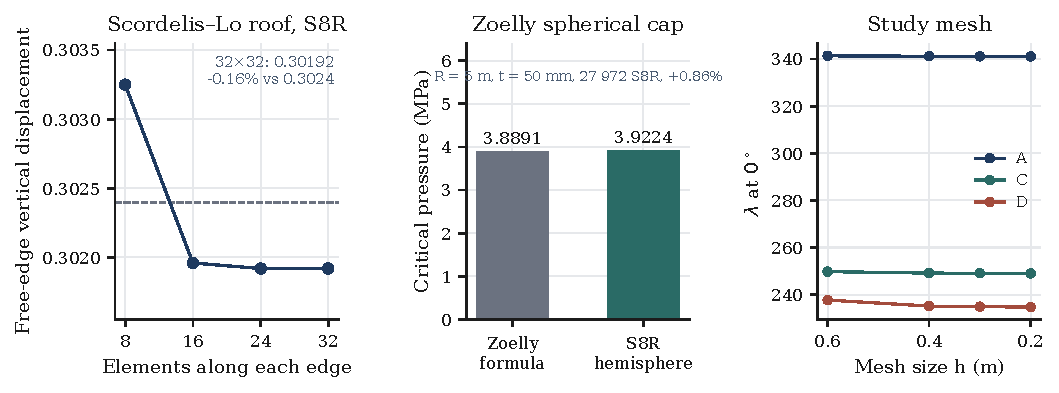
\includegraphics{figures/fig1_benchmarks.pdf}
\caption{Benchmarks behind Table~\ref{tab:benchmarks}.
Left: free-edge displacement of the Scordelis--Lo roof against 0.3024.
Centre: Zoelly pressure and the S8R hemisphere.
Right: \(\lambda\) at \(0^{\circ}\) for A, C and D as the mesh is refined.}
\label{fig:benchmarks}
\end{figure}

\section{Linear Eigenvalue Buckling Across Seven Equal-Volume Layouts}
\label{sec:linear}

Table~\ref{tab:layouts} and Figure~\ref{fig:layouts} give \(\lambda_c\) at \(V_{60}\), \(h = 0.4~\mathrm{m}\) and \(a_h = 0.20\).
The unrounded eigenvalues are 341.2093 for A, 395.9731 for B, 249.1289 for C, 235.0948 for D, 268.9580 for Dd, 193.1005 for Dx and 429.0206 for E.
Against A's 341.2093 these are \(+16.05\%\), \(-26.99\%\), \(-31.10\%\), \(-21.18\%\), \(-43.41\%\) and \(+25.74\%\).
The order is E, B, A, Dd, C, D, Dx.
Layout~E has no stored \(\lambda_g\).
Its reported factor is the lower of \(0^{\circ}\) and \(45^{\circ}\): 429.0206 at \(0^{\circ}\) and 438.0098 at \(45^{\circ}\).

The gain of E over A is 87.8113.
Recovery of that gain is \((\lambda-\lambda_A)/(\lambda_E-\lambda_A)\).
The orthogonal grid recovers 0.6237 of it, which is 62.37\%.
Layout~D is below A, so it recovers none: the stored ratio is \(-1.208\).
Layout~C is below A as well.
The registered statement, that D would recover at least 70\% of E's gain and that B and C would recover less than D, is not supported.

A, B, C, D and Dd stay within about 0.01\% around a square's symmetry orbit.
Dx, traced from \(+x\) only, runs from 193.1005 at \(0^{\circ}\) to 233.795 at \(180^{\circ}\).
That spread is 21.07\% of its \(\lambda_c\).
The worst direction in Table~\ref{tab:layouts} is \(180^{\circ}\) for A, C, D and Dd, and \(0^{\circ}\) for B and Dx.

On the uniform shell, \(\lambda_c/\lambda_g = 341.2093/369.7709 = 0.923\).
The same ratio at \(0.15g\), \(0.20g\), \(0.30g\) and \(0.40g\) is 0.943, 0.923, 0.884 and 0.849.
Sway at \(0.2g\) cuts the uniform-shell factor by about 8\%.
It does not dominate the buckling load.
At \(0.15g\), \(0.20g\) and \(0.30g\) the order of the seven \(V_{60}\) layouts is unchanged.
E is not re-optimised at the other accelerations.

Layout~B is the rib layout that beats A, and it is the layout that misses the volume.
The target is 9.669152~m\(^{3}\).
The meshed volume is 9.737968~m\(^{3}\), which is \(+0.712\%\).
The depth formula removes the 49 crossing footprints.
The element volume puts them back.
The \(+16.05\%\) is slightly on the heavy side of the equal-volume claim.
A, C, D, Dd, Dx and E match \(V_{60}\) to the stored digits.

The same layouts were recomputed from \(V/V_{60} = 1.0\) to 1.5, with E re-optimised at each volume by the six-variable \(D_4\) search.
C, D, Dd and Dx stay below A at every ratio, and their \(\lambda_c\) falls as the volume rises.
B stays above A.
From 1.1 to 1.3 times \(V_{60}\), B lies above the recorded \(D_4\) optimum.
The 25-zone search was not repeated away from \(V_{60}\), so the comparison at \(V/V_{60} = 1.2\), where B is 684.7 and the symmetric E is 546.9, is a comparison with the symmetric search only.

\begin{table}[t]
\centering
\caption{Equal-volume layouts at \(V_{60}\).
\(\lambda_c\) is the eight-direction minimum, except for E, where it is the minimum of \(0^{\circ}\) and \(45^{\circ}\).
\(\lambda_{\mathrm{GNIA}}\) is the minimum over \(L/300\), \(L/500\) and \(L/1000\) of the weaker sign, which is peak-down on every governing row.
For A, C and E that minimum is at \(L/500\).
For D it is at \(L/300\), so the \(-24.05\%\) is not a same-amplitude comparison.
The \(+15.02\%\) on E is \((135.96-118.20)/118.20\).
B, Dd and Dx were not run on the imperfect path.
B is 0.712\% above \(V_{60}\) in the mesh.}
\label{tab:layouts}
\small
\begin{tabular}{lrrrrl}
\toprule
Layout & $\lambda_c$ & vs.\ A & $\lambda_{\mathrm{GNIA}}$ & vs.\ A & Governing geometry \\
\midrule
A & 341.21 & baseline & 118.20 & baseline & uniform 60 mm \\
B & 395.97 & +16.05\% & n.a. & not run & 14 ribs, 62.4 mm, 49 crossings \\
C & 249.13 & -26.99\% & 91.30 & -22.76\% & 8 ribs, 157.6 mm, 0 crossings \\
D & 235.09 & -31.10\% & 89.77 & -24.05\% & 12 ribs, 208.8 mm, 0 crossings \\
Dd & 268.96 & -21.18\% & n.a. & not run & 8 ribs, 400.2 mm, 0 crossings \\
Dx & 193.10 & -43.41\% & n.a. & not run & 5 ribs, 505.1 mm, 0 crossings \\
E & 429.02 & +25.74\% & 135.96 & +15.02\% & 40.0--80.6 mm, 5 x 5 zones \\
\bottomrule
\end{tabular}

\end{table}

\begin{figure}[t]
\centering
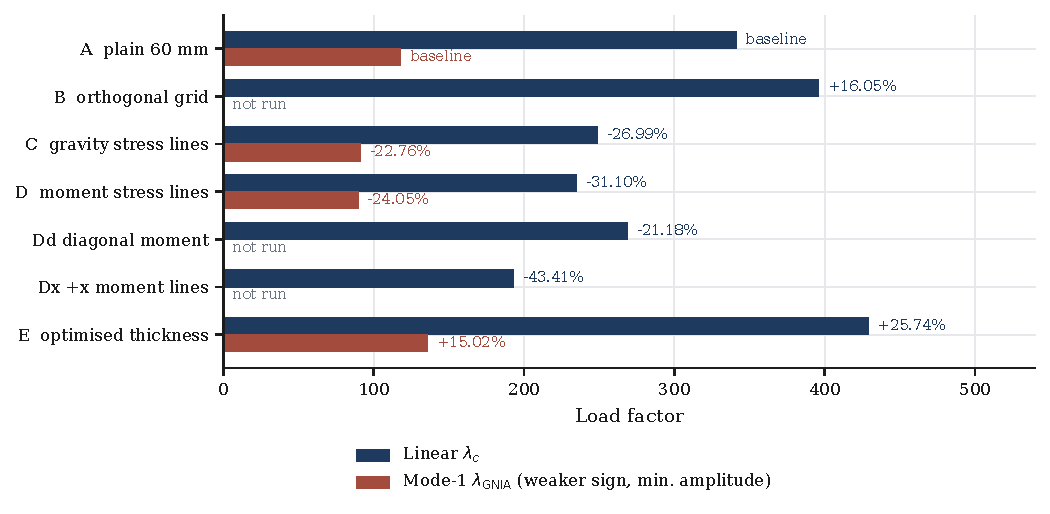
\includegraphics{figures/fig2_layout_buckling.pdf}
\caption{Linear factor \(\lambda_c\) for the seven layouts, and the governing mode-1 factor where the imperfect path was run.
The imperfect bars use the minimum over amplitude, as in Table~\ref{tab:layouts}.}
\label{fig:layouts}
\end{figure}

\section{Imperfection Sensitivity and Mechanical Failure Mechanism}
\label{sec:mechanism}

\subsection{Mode-1 paths}

\cite{koiter1945} showed that an unstable initial post-buckling path lets a small geometric imperfection cut the peak load, and \cite{hutchinson1967} showed how large that cut can be for a pressurised spherical shell.
Neither result is a knockdown factor for this roof.
The imperfection used here is one seeded mode, not a measured shape.

The imperfect calculations cover A, C, D and E only.
The first mode is scaled so that its largest translation equals \(w_0\).
With \(L = 12~\mathrm{m}\), the three amplitudes are \(L/300 = 0.040~\mathrm{m}\), \(L/500 = 0.024~\mathrm{m}\) and \(L/1000 = 0.012~\mathrm{m}\).
The sign called peak-down moves that node downwards.
Both signs are run.
The shape is the lower of the \(0^{\circ}\) and \(45^{\circ}\) eigenvalues.
For these four designs that angle is \(0^{\circ}\).
The linear factor stored beside D on the imperfect path is therefore the \(0^{\circ}\) value 235.1121, not the eight-direction minimum 235.0948.
The two differ by 0.017.
They are not mixed inside one percentage.

The weaker sign is peak-down on every governing row, and the classifier calls that row a limit point.
The other sign is often a solver stop.
Figure~\ref{fig:imperfection} plots both signs at \(L/500\), and the peak-down ratio \(\alpha = \lambda_{\mathrm{GNIA}}/\lambda_{\mathrm{LBA}}\) at the three amplitudes.
Load control cannot pass a limit point, and there is no Riks path.

At \(L/500\), peak-down, the imperfect factors are 118.202975 (A), 91.295285 (C), 98.291689 (D) and 135.958464 (E).
Against A, at that one amplitude, C is \(-22.76\%\), D is \(-16.84\%\) and E is \(+15.021\%\).
The order at matched amplitude is E, A, D, C.
The minimum over the three amplitudes is 118.202975 for A at \(L/500\), 91.295285 for C at \(L/500\), 89.771960 for D at \(L/300\), and 135.958464 for E at \(L/500\).
On those minima the order is E, A, C, D.
Table~\ref{tab:layouts} uses the minima.
D's \(-24.05\%\) in that table is 89.771960 against A's \(L/500\) factor, not against A at \(L/300\).

The published comparison of E with A uses \(L/500\) for both, which is also each design's minimum.
The unrounded ratio is
\begin{equation}
\frac{135.958464 - 118.202975}{118.202975} = +15.021\%.
\label{eq:gain}
\end{equation}
Rounded to two decimals first, \((135.96-118.20)/118.20 = +15.025\%\), which rounds to \(+15.03\%\).
Table~\ref{tab:layouts} prints \(+15.02\%\) for the same two-decimal pair.
The abstract uses \(+15.03\%\) for that rounded ratio, not for the unrounded \(+15.021\%\).
Whether \(L/500\) is the right reference amplitude for a code check is marked for the author to confirm.
B, Dd and Dx have no imperfect factor.

The ratio \(\alpha\) on the governing rows is 0.346 for A, 0.366 for C, 0.382 for D and 0.317 for E.
Across all twelve peak-down runs it lies between 0.317 and 0.503.
E is the most sensitive of the four on this ratio, and it remains the highest imperfect factor.
The linear gain of 25.74\% is reduced, not removed.
The stress-line layouts stay below the uniform shell on both the matched amplitude and the minimum over amplitude.

\begin{figure}[t]
\centering
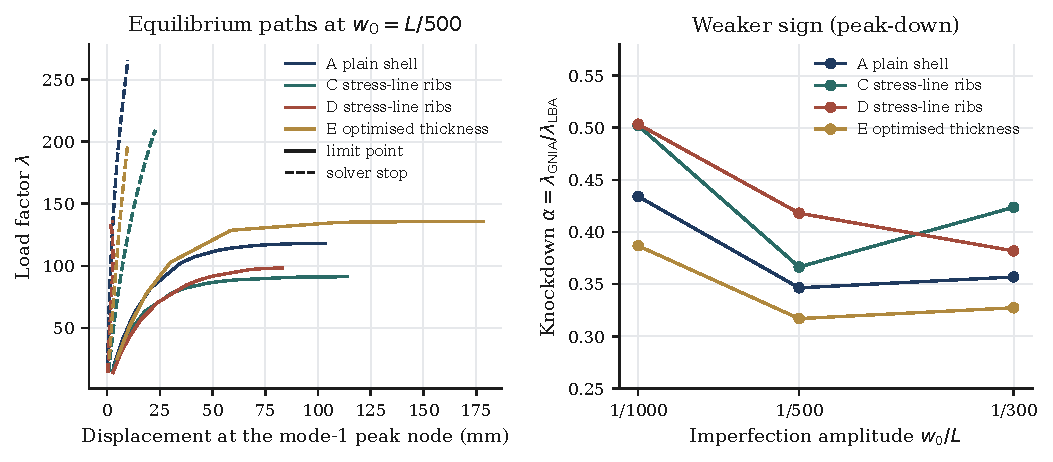
\includegraphics{figures/fig3_imperfection_sensitivity.pdf}
\caption{Mode-1 imperfect response of A, C, D and E.
Left: equilibrium paths at \(w_0 = L/500\), both signs.
A solid curve reaches a limit point.
A dashed curve is a solver stop and is not a buckling load.
Right: knockdown \(\alpha\) of the peak-down sign, which governs every design.}
\label{fig:imperfection}
\end{figure}

\subsection{Why the stress-line ribs lose capacity}

The loss is a stiffness result.
The model contains no cracking and no material failure, so it is not a fracture mechanism.

Layouts B to Dx buy their ribs by thinning the shell from 60~mm to 50~mm.
For an unreinforced panel, bending stiffness scales with \(t^{3}\) and membrane stiffness scales with \(t\).
A 50~mm panel therefore has \((50/60)^{3} = 0.5787\) of the bending stiffness of A, and \(5/6 = 0.8333\) of its membrane stiffness.
No modal split between membrane energy and bending energy is stored, so a shift from one to the other is not a measured result.
The scaling says only what the thinned panel is able to provide.

The stress-line layouts do not subdivide the bay.
C, D, Dd and Dx have no crossings.
Their spare volume, about one sixth of \(V_{60}\), sits in short, deep ribs.
D is twelve lines, 51.443~m, 208.8~mm deep.
B is the opposite geometry: fourteen lines, 179.469~m, 49 crossings, 1.5~m spacing, and only 62.4~mm of depth.
B is the rib layout that beats A.

A separate check at \(h = 0.6~\mathrm{m}\) and \(\theta = 0^{\circ}\) only asks whether the ribs are working.
It is not the study mesh and it is not the minimum over eight directions.
It was not run for B, Dd, Dx or E.
Figure~\ref{fig:mechanism} shows the six models.
The uniform 60~mm shell gives 341.41.
A bare 50~mm shell, with density scaled by \(60/50\) so that the weight equals \(V_{60}\), gives 221.23.
C at its equal-volume depth of 158~mm gives 249.75, which is 1.129 times the bare shell.
D at 209~mm gives 237.68, which is 1.074 times the bare shell.
Tripling the depth, without holding the volume, gives 227.56 for C (0.911 times that C, at 473~mm) and 179.92 for D (0.757 times that D, at 626~mm).

On the mode of that check, the largest displacement on a rib node is 0.370 of the shell peak for C and 0.409 for D.
The peak is in the shell.
The mean rib-node amplitude is 0.992 times the mean shell amplitude for C and 1.345 times for D, so the ribs of D are not nodal lines.
If the rib stiffness did not change and only the mass changed, an equal-volume shell (60~mm worth of material) against a shell with the rib volume tripled (80~mm worth) would give a factor \(0.060/0.080 = 0.75\).
The recorded 0.757 for D sits on that mass ratio.
Extra rib depth did not buy buckling stiffness.
The governing mode is panel buckling of the thinned shell between the ribs.
That reading matches the peak ratios and the mass-proportional drop.
It does not match a picture in which the ribs are quiet nodal lines.

E keeps one continuous shell.
At \(V_{60}\) the \(D_4\) optimum runs from the lower bound, 40.000~mm, to 80.629~mm.
Nine of the 25 zones sit on 40~mm.
The zones are 2.4~m square.
The largest step between zones that share an edge is 40.6~mm, a plan gradient of 0.0169.
The search objective is \(\lambda_c\).
It raises the factor from the uniform shell's 341.2094, the value stored as the start of that search, to 429.0206.
That is a redistribution of the same volume through the thickness.
It is not evidence about reinforcement, cracking, or a measured energy split.
Thickness redistribution is a standard variable in shell optimisation \citep{ramm1993}.
The result here is the equal-volume ranking against the rib layouts, not a transfer of those earlier examples.

\begin{figure}[t]
\centering
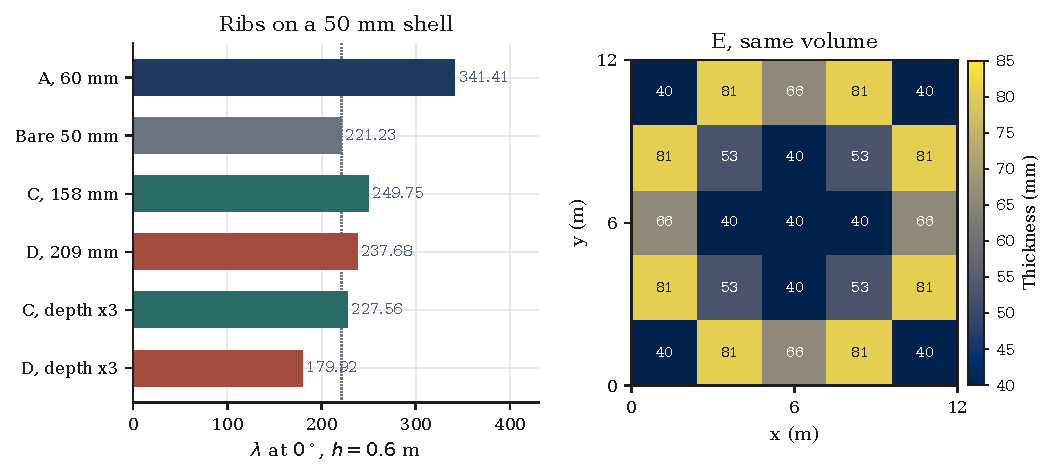
\includegraphics{figures/fig4_thickness_stiffness_mechanism.pdf}
\caption{Left: rib-depth check at \(h = 0.6~\mathrm{m}\) and \(\theta = 0^{\circ}\) only.
The bare 50~mm shell has its density scaled so that its weight matches \(V_{60}\).
Tripled depths are not equal-volume models.
Right: zone thickness of layout~E at the same volume.
Nine of the 25 zones lie on the 40~mm bound.}
\label{fig:mechanism}
\end{figure}

\section{Discussion: Fabrication Constraints, Embodied Carbon, and Limitations}
\label{sec:discussion}

The layouts that lose buckling capacity are also the layouts that are hardest to cast as drawn.
C has a minimum rib radius of 1.818~m.
D is 208.8~mm deep on a 50~mm shell, Dd is 400.2~mm deep, and Dx is 505.1~mm deep, with no crossings to brace the bay.
B is shallow, 62.4~mm, but it has 49 crossings and it is 0.712\% heavy.
E stays a continuous shell.
Its difficulty is the thickness step: 40.6~mm between zones that share an edge, on a 2.4~m grid, with nine zones held at the 40~mm bound that the search was allowed to reach.
None of these geometries was taken to a construction sequence or a physical model.

At one volume the concrete mass is one number.
For \(V_{60}\) it is \(9.669152495733323\times 2500 = 24172.9~\mathrm{kg}\).
The result file stores a carbon factor of 0.12~kgCO\(_{2}\)e/kg, with a low of 0.063 and a high of 0.149, and attributes the default to Table~2.3 of \cite{istructe2022} for UK in-situ C32/40 with 25\% ground granulated blast-furnace slag, taken from the ICE database.
The shell is called C30/37.
That table has no C30/37 row, and reinforcement is not included.
The factor is for the author to confirm.
With the stored default, the derived product-stage total is \(2.901~\mathrm{tCO_{2}e}\) at \(V_{60}\), and 1.523 to 3.602~t across the stored low and high factors.
Every layout that hits \(V_{60}\) has that same concrete total.
B is 0.712\% higher because it is 0.712\% heavier.
On this accounting, the layout that raises \(\lambda_c\) raises the buckling factor per unit of concrete carbon, and the stress-line ribs do not.
Giving them more concrete makes the linear factor worse: from \(V/V_{60} = 1.0\) to 1.5 their \(\lambda_c\) falls while they remain below A.
The missing reinforcement would add carbon to every ribbed layout and to any shell that needs steel to carry tension or to control cracking.
The stored factor does not price that steel, so the carbon comparison is a concrete comparison only.

The limitations of the model are the boundary of the result.

The material is linear-elastic and uncracked.
Cracking, reinforcement, creep, shrinkage and a long-term modulus are absent.
\cite{ramm1991} showed why that absence matters for a reinforced concrete shell: the ultimate load can be set by the interaction of large deformation and material failure, which this eigenvalue cannot see.

The lateral load is a constant acceleration on the mass, scaled with self-weight.
It is not a response spectrum and it is not a ground-motion history.
On the uniform shell it changes \(\lambda\) by about 8\% at \(0.2g\).
A corner-supported shell was screened and left out of the comparison because its sway ratio stayed above 0.91.

The imperfect analysis is one shape, mode~1, at one direction, at three amplitudes and two signs, and only for A, C, D and E.
Rib normals on the imperfect mesh are taken from the perfect surface.
There is one geometry, the rib depth is constant, there is no adjoint search over the rib layout, there are no construction stages, there is no code check, and there is no physical model.
The scope also asked for a bending moment under self-weight close to zero.
That number was not filed.

What the equal-volume ranking does support is a change in the next model, not a specification for a roof.
The elastic eigenvalue and one seeded mode are enough to reject stress-line ribs as a way to spend a fixed volume on this shell.
They are not enough to design the shell.
The open calculations are a nonlinear material and geometric analysis, in which cracking and reinforcement can move the limit load; a homogenised treatment of a ribbed surface, so that a grid can be judged without a beam-shell mesh that mis-counts crossings; and lightweight composite shells, for which both the volume constraint and the carbon factor are different from those of this concrete.

\section{Conclusion and Reproducibility Statement}
\label{sec:conclusion}

At the volume of a uniform 60~mm shell, moment stress-line ribs lose 31.10\% of the linear buckling factor under self-weight and a \(0.2g\) lateral body force.
A thickness field on the same shell, optimised for that factor, gains 25.74\%.
On the governing mode-1 path the same field gains 15.03\% when the two-decimal factors are ratioed, which is \(+15.021\%\) unrounded.
Gravity stress lines, the diagonal moment trace and the one-way moment trace also fall below the uniform shell.
An orthogonal grid gains 16.05\% and is 0.712\% over the target volume.
The registered recovery statement is not supported.
The ribs do not subdivide the bay, the shell that pays for them has 0.5787 of the uniform bending stiffness, and tripling the rib depth tracks the mass ratio.
The imperfect factors of A, C, D and E all lie well below their eigenvalues.
The thickness field remains the highest of the four.

The numbers are the stored CalculiX~2.23 results at commit \texttt{2025f66} on \texttt{main} (20~November 2026).
The jobs were not rerun for this note.
The repository is the link under the \mbox{author}.
Linear factors, the thickness optimum, the imperfect paths and the benchmarks are filed in \path{results/variants_h0.4_r1.json}, \path{results/E_best_d4_h0.4.json}, \path{results/gnia_h0.4.json} and \path{verify/out/}.
The author still has to confirm the tracing cut-offs, the mesh size, the use of \(L/500\) as a reference amplitude, and the carbon factor, which is a C32/40 row applied to a shell called C30/37 and which excludes reinforcement.

The next calculation is not another elastic ranking of these seven layouts.
It is a shell analysis in which the material can crack, the geometry can soften, a ribbed surface can be homogenised, and a lighter composite can be compared at its own mass and carbon.

\setlength{\bibsep}{2pt plus 1pt}
\bibliographystyle{plainnat}
\bibliography{refs}

\end{document}
